\documentclass[a4paper,12pt]{article}
\usepackage[russian]{babel}
\usepackage[utf8]{inputenc}
\usepackage{amsmath}
\usepackage{graphicx}
\usepackage[perpage]{footmisc} 
\usepackage{braket}
\usepackage{fullpage}
\newcommand{\vect}[1]{\boldsymbol{#1}}

% TODO
% Правки по Кукулину
% Таблицы 
% Координатное пр-во +1
% Результаты рассчетов +1
% Заключение +1
% Введение +1


\title{Высокоэнергетическое рассеяние без разложения по парциальным волнам.}
\author{.}

\begin{document}
	
	\maketitle
	\pagebreak
	%\setcounter{page}{2}
	
	\tableofcontents
    \pagebreak
     
	% \begin{abstract}
	% 	В данной работе получена конечномерная аппроксимация операторов рассеяния и уравнения Липпмана-Швингера путем перехода из базиса плоских волн в импульсное представление. В таком представлении функция Грина свободной частицы интегрируется аналитически, что существенно упрощает численное решение уравнений.
	% \end{abstract}
	% \pagebreak

	\section{Введение}
При энергиях порядка десятка МэВ вклад в процесс нуклон-нуклонного рассеяния даёт лишь небольшое количество парциальных амплитуд. В соответствии с этим разложение по парциальным волнам является адекватным методом расчета рассеяния. С другой стороны при энергиях порядка сотен МэВ и более возбуждается большие угловые моменты, которые дают вклад в амплитуду рассеяния. Такие вклады являются сильно осциллирующими функциями угла рассеяния при том, что результирующая амплитуда намного более гладкая функция.

Для решения возникающих при этом уравнений необходимы большие вычислительные мощности, и проведение таких расчетов на персональных компьютерах возможно лишь в небольшом числе случаев. В связи со все возрастающей доступностью параллельных вычислений (grid-сети, кластеры, суперкомпьютеры) возникает проблема разработки методов и алгоритмов решения задач рассеяния в многопоточном режиме. При этом возможно существенно увеличить число задач, поддающихся вычислению ab initio.

	\section{Базис стационарных волновых пакетов.}
Рассмотрим процесс рассеяния двух частиц. Гамильтониан этой системы запишем выделив взаимодействие и гамильтониан свободной частицы:
\[
	H = H_0 + V,
\]
где потенциал $V$ – короткодействующий с характерным размером $a$. Собственные функции $H_0$ это состояния с определенным импульсом, выберем их нормированными на дельта-функцию:
\[
	\braket{\vect{r}|\vect{q}} = \frac{1}{(2\pi)^{3/2}}e^{i\vect{q}\vect{r}} 
\]\[
	\braket{\vect{q}|\vect{q'}} = \delta(\vect{q} - \vect{q'})
\]

%	\subsection{Волновые пакеты.}
Перейдем от точных волновых функций к стационарным волновым пакетам. Введем разбиение $D$ трехмерного импульсного пространства на малые области и перенумеруем эти области индексом $\alpha$. Волновым пакетом мы будем называть сумму всех $\ket{\vect{q}}$, импульс которых попадает в заданную область $D_\alpha$. При этом интегрирование произведем с весовой функцией $f(q)$ смысл которой будет объяснен далее:
\[
	\ket{\alpha} = \frac{1}{\sqrt{\mu_\alpha}} \int\limits_{D_\alpha} f(q) \ket{\vect{q}} d^3q
\]
Коэффициент $\mu_\alpha$ найдем из условия нормировки:
\[
	\braket{\alpha|\beta} = \frac{1}{\sqrt{\mu_\alpha \mu_\beta}}  \int\limits_{D_\alpha}  \int\limits_{D_\beta} f(q)f^\dagger(q') \delta(\vect{q} - \vect{q'}) d^3q d^3q' = 1
\]
Отсюда имеем:
\[
	\mu_\alpha =  \int\limits_{D_\alpha} |f(q)|^2 d^3q
\]
Таким образом мы заменили непрерывный спектр на квазидискретный и полученный набор функций является ортонормированным. Полным этот набор функций становится в пределе $D_\alpha \to 0$:
\[
	\braket{\alpha|\beta} = \delta_{\alpha,\beta}
\]\[
	\sum\limits_\alpha \ket{\alpha}\bra{\alpha} = P
\]

Сетку разбиения удобно выбирать так, чтобы её поверхности уровня совпадали с поверхностями уровня системы координат в которых производится интегрирование. Например, если $d^3q = dq_xdq_ydq_z$, то логично выбрать прямоугольную решетку. Более же удобным в данном случае будет интегрирование в сферической системе координат, во-первых энергия зависит только от одной координаты – модуля импульса, во-вторых явно выделен азимутальный угол и это существенно упростит решение задач со сферически-симметричным потенциалом. Таким образом $D_\alpha$ это следующая область:
\[
 D_{\alpha(i,j,k)} = \big\{ \: (k,\theta,\varphi) \: \big| \: q \in [q_i,q_{i+1}], \theta \in [\theta_j,\theta_{j+1}], \varphi \in [\varphi_k,\varphi_{k+1}] \: \big\} 
\]\[
 \alpha \text{ нумерует сочетания } \big\{ (0,0,0), \; ... \; , (i_{max},j_{max},k_{max}) \big\}
\]

	\subsection{Волновые пакеты в случае аксиальной симметрии.}
В случае сферически-симмеричного потенциала результат решения задачи не должен зависеть от азимутального угла. При этом удобно использовать смешанное представление, в котором угол $\varphi$ – непрерывная переменная, а модуль $|\vect{q}|$ и полярный угол – дискретные. Интегрирование проведем в сферических координатах. Итого, имеем следующее представление:

\[
	\ket{\alpha,\varphi} = \frac{1}{\sqrt{\mu_\alpha}} \int\limits_{D_\alpha} f(q) \ket{\vect{q}} q^2 \,dq \,d(-\cos\theta)
\]
\[
	\mu_\alpha =  \int\limits_{D_\alpha} |f(q)|^2 q^2 \,dq \,d(-\cos\theta)
\]
Определенные так волновые пакеты нормированны следующим условием:
\[
	\braket{\alpha,\varphi|\beta,\varphi'} = \delta_{\alpha,\beta}\delta(\varphi'-\varphi)
\]\[
	\sum\limits_\alpha \int\limits_0^{2\pi} \,d \varphi \ket{\alpha,\varphi}\bra{\alpha,\varphi} = 1
\]
Теперь рассмотрим подробнее решетку:
\[
 \text{ узлы решетки по }q: \;\; q_i, \;\;\; i=\overline{0,M}
\]\[
 \text{ узлы решетки по }\theta: \;\;  \theta_j, \;\;\; j=\overline{0,N}
\]
На каждом интервале выберем средний элемент
\[
 q_i^* \in [q_i,q_{i+1}], \;\;\; i=\overline{0,M-1}
\]\[
 \theta_j^* \in [\theta_j,\theta_{j-1}], \;\;\; j=\overline{0,N-1}
\]
и перейдем от двойного индекса $(i,j)$ к одинарному
\[
	\alpha = \overline{0,N M-1},
\]\[
	i = [\alpha/N], \;\;\; j = \alpha \bmod N,
\]\[
	\vect{q^*_\alpha} = (q_i^*,\theta_j^*),
\]
где $x \bmod y$ – остаток от деления $x$ на $y$, а $[x/y]$ – целая часть деления. Если рассматривать величины $(q_i^*,\theta_j^*)$ как элементы матрицы, то такое преобразование эквивалетно следующему изменению индексов в матрице:
\[
\begin{pmatrix} 
a_{00}    & a_{01}    & \dots  & a_{0,N-1}  \\ 
a_{10}    & a_{11}    & \dots  & a_{1,N-1}  \\ 
\vdots    & \vdots    & \ddots & \vdots     \\ 
a_{M-1,0} & a_{M-1,1} & \dots  & a_{M-1,N-1}  
\end{pmatrix}  \longrightarrow  \begin{pmatrix} 
a_{0}      & a_{1}        & \dots   & a_{N-1}  \\  
a_{N}      & a_{N+1}      & \dots   & a_{2N-1} \\ 
\vdots     & \vdots       & \ddots  & \vdots   \\
a_{(M-1)N} & a_{(M-1)N+1} & \dots   & a_{NM-1} 
\end{pmatrix}
\]

\subsection{Операторы в представлении Волновых Пакетов.}

Теперь получим выражение операторов в представлении Волновых Пакетов (ВП) через операторы в импульсном представлении. Пусть дан оператор с матричными элементами в импульсном представлении
\[
	A(\vect{q'},\vect{q}) \equiv \bra{\vect{q'}}A\ket{\vect{q}}
\] и оператор с матричными элементами в представлении ВП \[
  A_{\alpha\beta}(\varphi',\varphi) \equiv \bra{\alpha,\varphi'}A\ket{\beta,\varphi}.
\]
Переход от одного представления к другому осуществляется по стандартной формуле:
\[
	A_{\alpha\beta}(\varphi',\varphi) = \int d^3q \int d^3q' \braket{\alpha,\varphi'|\vect{q'}} A(\vect{q'},\vect{q}) \braket{\vect{q}|\beta,\varphi}.
\] 
Перекрывание ВП и плоской волны вычисляется исходя из определения ВП:
\[
 \braket{\vect{q}|\alpha,\varphi'} = \frac{f(q)}{\sqrt{\mu_\alpha}} \delta_{\alpha,\{\vect{q}\}} \delta(\varphi'-\varphi)
\]
Здесь и далее под $\{\vect{q}\}$ подразумевается номер интервала в который попадает этот вектор. Подставляя это в интеграл перехода получим:
\[
 A_{\alpha\beta}(\varphi',\varphi) = \frac{1}{\sqrt{\mu_\alpha \mu_\beta}} \int\limits_{D_\alpha} f^\dagger(q) d^2q \int\limits_{D_\beta} f(q') d^2q' A(\vect{q'},\vect{q})
\] Пользуясь теоремой о среднем и малостью интервала интегрирования выносим $A(\vect{q'},\vect{q})$ за знак интеграла:
\[
 A_{\alpha\beta}(\varphi',\varphi) = \frac{A(\vect{q^*_\alpha},\vect{q^*_\beta})}{\sqrt{\mu_\alpha \mu_\beta}} \int\limits_{D_\alpha} f^\dagger(q) d^2q \int\limits_{D_\beta} f(q') d^2q'
\] Оставшиеся два интеграла также пользуясь теоремой о среднем можно привести к виду нормировочных интегралов. И окончательный результат:
\[
 A_{\alpha\beta}(\varphi',\varphi) = \frac{\sqrt{\mu_\alpha \mu_\beta}}{ f^\dagger(q_\alpha^*)f(q_\beta^*) }  A(\vect{q^*_\alpha},\vect{q^*_\beta}).
\]
Все операторы рассеяния будут выражаться через велечины $A(\vect{q^*_\alpha},\vect{q^*_\beta})$ поэтому введем для них краткие обозначения:
\begin{equation}
    \label{mesh_oper}
    A(\vect{q^*_\alpha},\vect{q^*_\beta}) \equiv A^*_{\alpha\beta}
\end{equation}

\subsection{Поведение ВП в координатном пространстве.}
-- Рассмотреть при разных $f(q)$ --




\section{Уравнение Липпмана-Швингера.}

Двухчастичное рассеяние описывается уравнением Липпмана-Швингера
\begin{equation}
    T = V + V G_0 T,
\end{equation}
где $V$ — двухчастичный потенциал, $G_0 = (z - H_0)^{-1}$ — функция Грина свободной частицы и $T$ это T-матрица. В импульсном пространстве матричные элементы $T(\vect{q'},\vect{q},z) \equiv \bra{\vect{q'}}T(z)\ket{\vect{q}}$  удовлетворяют интегральному уравнению
\begin{equation}
    T(\vect{q'},\vect{q}, z) = V(\vect{q'},\vect{q}) + \int d^3q'' V(\vect{q'},\vect{q''}) G_0(\vect{q''},z) T(\vect{q''},\vect{q}, z). 
\end{equation}
Здечь $\vect{q}$ это относительный импульс, $m$ — приведенная масса двух частиц и $z$ это энергия. Мы рассматриваем нерелятивистский случай и ограничемся двумя бесспиновыми частицами. Таким образом $V(\vect{q'},\vect{q})$ и $T(\vect{q'},\vect{q},z)$ являются скалярными функциями:
\begin{equation}
    V(\vect{q'},\vect{q}) = V(q',q,\vect{q'}\vect{q})
\end{equation}
и
\begin{equation}
    T(\vect{q'},\vect{q}) = T(q',q,\vect{q'}\vect{q})
\end{equation}
В последнем выражении мы отбосили параметрическую зависимость от $z$. Рассмотрим теперь как выражаются операторы в представлении волновых пакетов через операторы в импульсном представлении.


\subsection{Функция Грина в представлении ВП.}
Действуя на функцию Грина свободной частицы
\[
	G(q_0) = \frac{2m}{\hbar^2} \int d^3q \frac{ \ket{\vect{q}} \bra{ \vect{q} } }{ q_0^2 - q^2 + i\epsilon } 
\]
операторами проектирования
\[
	P = \sum\limits_\alpha \int\limits_0^{2\pi} \,d \varphi \ket{\alpha,\varphi}\bra{\alpha,\varphi}
\] 
с двух сторон, получим функцию Грина в представлении ВП:

\[
  G(q_0) = 
	\frac{2m}{\hbar^2}  \sum\limits_\alpha \frac{1}{ \mu_\alpha } \int\limits_{D_\alpha} d^3q 
		\frac{ \ket{\alpha,\varphi} |f(q)|^2 \bra{\alpha,\varphi} }{ q_0^2 - q^2 + i\epsilon } 
\]
Рассматривая $\alpha$-ый элемент этой суммы, вводя сферические координаты и интегрируя по $\varphi$ и $\theta$ имеем:
\[
  G_\alpha = \frac{2m (cos(\theta_j^*)-cos(\theta_{j+1}^*))}{\hbar^2 \mu_\alpha} \int\limits_{\Delta q_i}
		\frac{ |f(q)|^2 q^2 dq }{ q_0^2 - q^2 + i\epsilon } 
\]
и окончательно в случае $f(q)=1$:
\begin{equation}
  \label{greene1}
  G_\alpha = \frac{2m}{\hbar^2} \frac{cos(\theta_j^*)-cos(\theta_{j+1}^*)}{\mu_\alpha}
		\bigg( 
			q_{i+1}^* - q_i^* + \frac{q_0}{2}\ln\frac{(q_{i+1}^* +q_0)(q_i^* -q_0)}{(q_{i+1}^* -q_0)(q_i^* +q_0)} + \frac{i\pi q_0}{2}\delta_{\{q'\},i}
		\bigg)
\end{equation}
и в случае $f(q)=1/q$:
\begin{equation}
  \label{greene2}
  G_\alpha = \frac{2m}{\hbar^2} \frac{cos(\theta_j^*)-cos(\theta_{j+1}^*)}{\mu_\alpha} 
		\bigg( 
			\frac{q_0}{2}\ln\frac{(q_{i+1}^* +q_0)(q_i^* -q_0)}{(q_{i+1}^* -q_0)(q_i^* +q_0)} + \frac{i\pi q_0}{2}\delta_{\{q'\},i}
		\bigg)
\end{equation}
Так же как и для операторов в формуле (\ref{mesh_oper}) для функции Грина введем обозначения
\begin{equation}
    \label{mesh_greene}
    G_\alpha = \frac{cos(\theta_j^*)-cos(\theta_{j+1}^*)}{\mu_\alpha} G^*_\alpha
\end{equation} где $G^*_\alpha$ можно найти сравнивая с формулами (\ref{greene1}) и (\ref{greene2}).


\subsection{Уравнение Липпманна-Швингера в представлении ВП.}

Используя результаты пункта 2.3 запишем в представлении ВП Т-матрицу:
\begin{equation}
	T_{\alpha\beta}(\varphi,\varphi') = \frac{\sqrt{\mu_\alpha \mu_\beta}}{ f^\dagger(q_\alpha^*)f(q_\beta^*) } T(\vect{q^*_\alpha},\vect{q^*_\beta})
\end{equation}
и аналагично потенциал.

Запишем теперь уравнение Липпманна-Швингера в представлении ВП:
\begin{equation}
 T_{\alpha\alpha_0}(\varphi-\varphi_0) = 
 V_{\alpha\alpha_0}(\varphi-\varphi_0) + 
 \sum\limits_\beta \int\limits_0^{2\pi} d \varphi' V_{\alpha\beta}(\varphi-\varphi') G_{\beta} T_{\beta\alpha_0}(\varphi'-\varphi_0)
\end{equation}
где $\alpha_0$ и $\varphi_0$ - координаты $\vect{q_0}$.  Так как потенциал сферически-симметричный Т-матрица не может зависить от $\varphi$. Зависимость от этого угла есть только в потенциале и имеет следующий вид:
\begin{equation}
\label{pifagor_3d}
    V(\vect{q'},\vect{q}) = V(q',q, \cos(\theta')\cos(\theta) + \sin(\theta')\sin(\theta)\cos(\varphi) )
\end{equation} 
Поэтому можем провести интегрирование по $\varphi$ и ввести новую функцию:
\begin{equation}
    \label{phi_int}
    W_{\alpha\beta} = \int\limits_{0}^{2\pi} d\varphi V_{\alpha\beta}(\varphi)
\end{equation}
Если один из индексов отвечает импульсу налетающей частицы, то можно проинтегрировать явно, так как зависимость от $\varphi$ в выражении (\ref{pifagor_3d}) исчезает.
\begin{equation}
    V_{\alpha\alpha_0} = \frac{1}{2\pi}W_{\alpha\alpha_0}
\end{equation}

Тогда уравнение принимает вид
\begin{equation}
    T_{\alpha\alpha_0} = \frac{1}{2\pi}W_{\alpha\alpha_0} + \sum\limits_\beta  W_{\alpha\beta} G_{\beta} T_{\beta\alpha_0}
\end{equation}
Используя формулы (\ref{mesh_oper}), (\ref{mesh_greene}) и сокращая нормировочные множители, получим явный вид данного уавнения:
\begin{equation}
    T^*_{\alpha\alpha_0} = \frac{1}{2\pi}W^*_{\alpha\alpha_0} +
 \sum\limits_\beta \frac{cos(\theta_j^*)-cos(\theta_{j+1}^*)}{|f_\beta|^2} W^*_{\alpha\beta} G^*_{\beta} T^*_{\beta\alpha_0}
\end{equation}

Решив уравнение Липпманна-Швингера получим матричные элементы Т-оператора. Они прямо пропорциональны амплитуде рассеяния. Учитывая сохранение импульса имеем:
\begin{equation}
    f_t = - \frac{2m}{\hbar^2} \frac{(2\pi)^2}{2} T^*_{\alpha\alpha_0},
\end{equation}
где $\alpha \in {\alpha_0, ... , \alpha_0 + N}$, а $t \in {0, ... ,N} $.




%\section{Поведение высших борновских членов}
\section{Численные иллюстрации}
Для иллюстрации полученного метода произведен расчет сечения рассеяния для двух потенциалов. В обоих случаях результаты сравнивались с методом парциальных волн, который выбран за эталонный.


	\subsection{Расчет для Гауссова потенциала.}
	В качестве простого теста используем потенциал в виде гауссового пика.
	\begin{equation}
	   V(r) = A e^{-r^2/a^2},
	\end{equation}
	и соостветственно
	\begin{equation}
	   V(\vect{q'},\vect{q}) = \frac{Aa^3}{8\pi^{3/2}}\exp\big( - \frac{a^2}{4}(\vect{q'}-\vect{q})^2 \big)
	\end{equation}
	Интегрирование по $\varphi$ в соответствии с (\ref{phi_int}) может быть проведено аналитически
	\begin{equation}
	   W(\vect{q_2},\vect{q_1}) = \frac{Aa^3}{4\pi^{1/2}} e^{ - a^2( q_1^2 + q_2^2 - 2q_1q_2\cos\theta_1\cos\theta_2)/4 }
	    I_0 \big( a^2q_1q_2\sin\theta_1\sin\theta_2/2 \big)
	\end{equation}
	где $I_0$ -- модифицированная функция Бесселя.
	
	Результаты сравним с методом волновых функций.
	
	
	
	\subsection{Расчет для потенциала Малфлье-Тьёна.}

\section{Заключение}

    \pagebreak
    \subsection{Таблицы}
    %таблицы

    
    \pagebreak
    \subsection{Приложение 1. Рассеяние на Гауссовом потенциале.}
    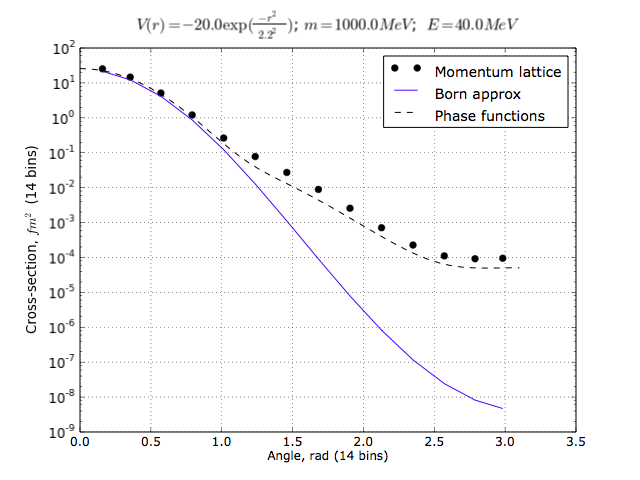
\includegraphics[width=150mm]{gauss-high.png}
    \newline
    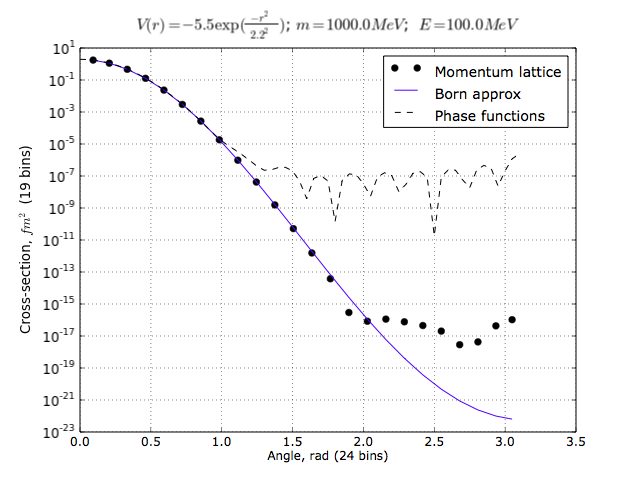
\includegraphics[width=150mm]{gauss-low.png}
    
    \pagebreak
    \subsection{Приложение 2. Рассеяние на потенциале Малфлье-Тьёна.}

    
    \pagebreak
    \subsection{Приложение 3. Поведение высших борновских членов.}

    
\end{document}

